% IEEEtran V1.7 and later provides for these CLASSINPUT macros to allow the
% user to reprogram some IEEEtran.cls defaults if needed. These settings
% override the internal defaults of IEEEtran.cls regardless of which class
% options are used. Do not use these unless you have good reason to do so as
% they can result in nonIEEE compliant documents. User beware. ;)
%
%\newcommand{\CLASSINPUTbaselinestretch}{1.0} % baselinestretch
%\newcommand{\CLASSINPUTinnersidemargin}{1in} % inner side margin
%\newcommand{\CLASSINPUToutersidemargin}{1in} % outer side margin
%\newcommand{\CLASSINPUTtoptextmargin}{1in}   % top text margin
%\newcommand{\CLASSINPUTbottomtextmargin}{1in}% bottom text margin


%
\documentclass[10pt,journal,compsoc]{IEEEtran}
% If IEEEtran.cls has not been installed into the LaTeX system files,
% manually specify the path to it like:
% \documentclass[10pt,journal,compsoc]{../sty/IEEEtran}


% Some very useful LaTeX packages include:
% (uncomment the ones you want to load)


% *** MISC UTILITY PACKAGES ***
%
%\usepackage{ifpdf}
% Heiko Oberdiek's ifpdf.sty is very useful if you need conditional
% compilation based on whether the output is pdf or dvi.
% usage:
% \ifpdf
%   % pdf code
% \else
%   % dvi code
% \fi
% The latest version of ifpdf.sty can be obtained from:
% http://www.ctan.org/pkg/ifpdf
% Also, note that IEEEtran.cls V1.7 and later provides a builtin
% \ifCLASSINFOpdf conditional that works the same way.
% When switching from latex to pdflatex and vice-versa, the compiler may
% have to be run twice to clear warning/error messages.


% *** CITATION PACKAGES ***
%
\ifCLASSOPTIONcompsoc
  % The IEEE Computer Society needs nocompress option
  % requires cite.sty v4.0 or later (November 2003)
  \usepackage[nocompress]{cite}
\else
  % normal IEEE
  \usepackage{cite}
\fi
% cite.sty was written by Donald Arseneau
% V1.6 and later of IEEEtran pre-defines the format of the cite.sty package
% \cite{} output to follow that of the IEEE. Loading the cite package will
% result in citation numbers being automatically sorted and properly
% "compressed/ranged". e.g., [1], [9], [2], [7], [5], [6] without using
% cite.sty will become [1], [2], [5]--[7], [9] using cite.sty. cite.sty's
% \cite will automatically add leading space, if needed. Use cite.sty's
% noadjust option (cite.sty V3.8 and later) if you want to turn this off
% such as if a citation ever needs to be enclosed in parenthesis.
% cite.sty is already installed on most LaTeX systems. Be sure and use
% version 5.0 (2009-03-20) and later if using hyperref.sty.
% The latest version can be obtained at:
% http://www.ctan.org/pkg/cite
% The documentation is contained in the cite.sty file itself.
%
% Note that some packages require special options to format as the Computer
% Society requires. In particular, Computer Society  papers do not use
% compressed citation ranges as is done in typical IEEE papers
% (e.g., [1]-[4]). Instead, they list every citation separately in order
% (e.g., [1], [2], [3], [4]). To get the latter we need to load the cite
% package with the nocompress option which is supported by cite.sty v4.0
% and later.


% *** GRAPHICS RELATED PACKAGES ***
%
\ifCLASSINFOpdf
  \usepackage[pdftex]{graphicx}
  % declare the path(s) where your graphic files are
  % \graphicspath{{../pdf/}{../jpeg/}}
  % and their extensions so you won't have to specify these with
  % every instance of \includegraphics
  % \DeclareGraphicsExtensions{.pdf,.jpeg,.png}
\else
  % or other class option (dvipsone, dvipdf, if not using dvips). graphicx
  % will default to the driver specified in the system graphics.cfg if no
  % driver is specified.
  % \usepackage[dvips]{graphicx}
  % declare the path(s) where your graphic files are
  % \graphicspath{{../eps/}}
  % and their extensions so you won't have to specify these with
  % every instance of \includegraphics
  % \DeclareGraphicsExtensions{.eps}
\fi
% graphicx was written by David Carlisle and Sebastian Rahtz. It is
% required if you want graphics, photos, etc. graphicx.sty is already
% installed on most LaTeX systems. The latest version and documentation
% can be obtained at: 
% http://www.ctan.org/pkg/graphicx
% Another good source of documentation is "Using Imported Graphics in
% LaTeX2e" by Keith Reckdahl which can be found at:
% http://www.ctan.org/pkg/epslatex
%
% latex, and pdflatex in dvi mode, support graphics in encapsulated
% postscript (.eps) format. pdflatex in pdf mode supports graphics
% in .pdf, .jpeg, .png and .mps (metapost) formats. Users should ensure
% that all non-photo figures use a vector format (.eps, .pdf, .mps) and
% not a bitmapped formats (.jpeg, .png). The IEEE frowns on bitmapped formats
% which can result in "jaggedy"/blurry rendering of lines and letters as
% well as large increases in file sizes.
%
% You can find documentation about the pdfTeX application at:
% http://www.tug.org/applications/pdftex


% *** MATH PACKAGES ***
%
%\usepackage{amsmath}
% A popular package from the American Mathematical Society that provides
% many useful and powerful commands for dealing with mathematics.
%
% Note that the amsmath package sets \interdisplaylinepenalty to 10000
% thus preventing page breaks from occurring within multiline equations. Use:
%\interdisplaylinepenalty=2500
% after loading amsmath to restore such page breaks as IEEEtran.cls normally
% does. amsmath.sty is already installed on most LaTeX systems. The latest
% version and documentation can be obtained at:
% http://www.ctan.org/pkg/amsmath


% *** SPECIALIZED LIST PACKAGES ***
%\usepackage{acronym}
% acronym.sty was written by Tobias Oetiker. This package provides tools for
% managing documents with large numbers of acronyms. (You don't *have* to
% use this package - unless you have a lot of acronyms, you may feel that
% such package management of them is bit of an overkill.)
% Do note that the acronym environment (which lists acronyms) will have a
% problem when used under IEEEtran.cls because acronym.sty relies on the
% description list environment - which IEEEtran.cls has customized for
% producing IEEE style lists. A workaround is to declared the longest
% label width via the IEEEtran.cls \IEEEiedlistdecl global control:
%
% \renewcommand{\IEEEiedlistdecl}{\IEEEsetlabelwidth{SONET}}
% \begin{acronym}
%
% \end{acronym}
% \renewcommand{\IEEEiedlistdecl}{\relax}% remember to reset \IEEEiedlistdecl
%
% instead of using the acronym environment's optional argument.
% The latest version and documentation can be obtained at:
% http://www.ctan.org/pkg/acronym


%\usepackage{algorithmic}
% algorithmic.sty was written by Peter Williams and Rogerio Brito.
% This package provides an algorithmic environment fo describing algorithms.
% You can use the algorithmic environment in-text or within a figure
% environment to provide for a floating algorithm. Do NOT use the algorithm
% floating environment provided by algorithm.sty (by the same authors) or
% algorithm2e.sty (by Christophe Fiorio) as the IEEE does not use dedicated
% algorithm float types and packages that provide these will not provide
% correct IEEE style captions. The latest version and documentation of
% algorithmic.sty can be obtained at:
% http://www.ctan.org/pkg/algorithms
% Also of interest may be the (relatively newer and more customizable)
% algorithmicx.sty package by Szasz Janos:
% http://www.ctan.org/pkg/algorithmicx



% *** ALIGNMENT PACKAGES ***
%
%\usepackage{array}
% Frank Mittelbach's and David Carlisle's array.sty patches and improves
% the standard LaTeX2e array and tabular environments to provide better
% appearance and additional user controls. As the default LaTeX2e table
% generation code is lacking to the point of almost being broken with
% respect to the quality of the end results, all users are strongly
% advised to use an enhanced (at the very least that provided by array.sty)
% set of table tools. array.sty is already installed on most systems. The
% latest version and documentation can be obtained at:
% http://www.ctan.org/pkg/array


%\usepackage{mdwmath}
%\usepackage{mdwtab}
% Also highly recommended is Mark Wooding's extremely powerful MDW tools,
% especially mdwmath.sty and mdwtab.sty which are used to format equations
% and tables, respectively. The MDWtools set is already installed on most
% LaTeX systems. The lastest version and documentation is available at:
% http://www.ctan.org/pkg/mdwtools


% IEEEtran contains the IEEEeqnarray family of commands that can be used to
% generate multiline equations as well as matrices, tables, etc., of high
% quality.


%\usepackage{eqparbox}
% Also of notable interest is Scott Pakin's eqparbox package for creating
% (automatically sized) equal width boxes - aka "natural width parboxes".
% Available at:
% http://www.ctan.org/pkg/eqparbox


% *** SUBFIGURE PACKAGES ***
%\ifCLASSOPTIONcompsoc
%  \usepackage[caption=false,font=footnotesize,labelfont=sf,textfont=sf]{subfig}
%\else
%  \usepackage[caption=false,font=footnotesize]{subfig}
%\fi
% subfig.sty, written by Steven Douglas Cochran, is the modern replacement
% for subfigure.sty, the latter of which is no longer maintained and is
% incompatible with some LaTeX packages including fixltx2e. However,
% subfig.sty requires and automatically loads Axel Sommerfeldt's caption.sty
% which will override IEEEtran.cls' handling of captions and this will result
% in non-IEEE style figure/table captions. To prevent this problem, be sure
% and invoke subfig.sty's "caption=false" package option (available since
% subfig.sty version 1.3, 2005/06/28) as this is will preserve IEEEtran.cls
% handling of captions.
% Note that the Computer Society format requires a sans serif font rather
% than the serif font used in traditional IEEE formatting and thus the need
% to invoke different subfig.sty package options depending on whether
% compsoc mode has been enabled.
%
% The latest version and documentation of subfig.sty can be obtained at:
% http://www.ctan.org/pkg/subfig


% *** FLOAT PACKAGES ***
%
%\usepackage{fixltx2e}
% fixltx2e, the successor to the earlier fix2col.sty, was written by
% Frank Mittelbach and David Carlisle. This package corrects a few problems
% in the LaTeX2e kernel, the most notable of which is that in current
% LaTeX2e releases, the ordering of single and double column floats is not
% guaranteed to be preserved. Thus, an unpatched LaTeX2e can allow a
% single column figure to be placed prior to an earlier double column
% figure.
% Be aware that LaTeX2e kernels dated 2015 and later have fixltx2e.sty's
% corrections already built into the system in which case a warning will
% be issued if an attempt is made to load fixltx2e.sty as it is no longer
% needed.
% The latest version and documentation can be found at:
% http://www.ctan.org/pkg/fixltx2e


%\usepackage{stfloats}
% stfloats.sty was written by Sigitas Tolusis. This package gives LaTeX2e
% the ability to do double column floats at the bottom of the page as well
% as the top. (e.g., "\begin{figure*}[!b]" is not normally possible in
% LaTeX2e). It also provides a command:
%\fnbelowfloat
% to enable the placement of footnotes below bottom floats (the standard
% LaTeX2e kernel puts them above bottom floats). This is an invasive package
% which rewrites many portions of the LaTeX2e float routines. It may not work
% with other packages that modify the LaTeX2e float routines. The latest
% version and documentation can be obtained at:
% http://www.ctan.org/pkg/stfloats
% Do not use the stfloats baselinefloat ability as the IEEE does not allow
% \baselineskip to stretch. Authors submitting work to the IEEE should note
% that the IEEE rarely uses double column equations and that authors should try
% to avoid such use. Do not be tempted to use the cuted.sty or midfloat.sty
% packages (also by Sigitas Tolusis) as the IEEE does not format its papers in
% such ways.
% Do not attempt to use stfloats with fixltx2e as they are incompatible.
% Instead, use Morten Hogholm'a dblfloatfix which combines the features
% of both fixltx2e and stfloats:
%
% \usepackage{dblfloatfix}
% The latest version can be found at:
% http://www.ctan.org/pkg/dblfloatfix


%\ifCLASSOPTIONcaptionsoff
%  \usepackage[nomarkers]{endfloat}
% \let\MYoriglatexcaption\caption
% \renewcommand{\caption}[2][\relax]{\MYoriglatexcaption[#2]{#2}}
%\fi
% endfloat.sty was written by James Darrell McCauley, Jeff Goldberg and 
% Axel Sommerfeldt. This package may be useful when used in conjunction with 
% IEEEtran.cls'  captionsoff option. Some IEEE journals/societies require that
% submissions have lists of figures/tables at the end of the paper and that
% figures/tables without any captions are placed on a page by themselves at
% the end of the document. If needed, the draftcls IEEEtran class option or
% \CLASSINPUTbaselinestretch interface can be used to increase the line
% spacing as well. Be sure and use the nomarkers option of endfloat to
% prevent endfloat from "marking" where the figures would have been placed
% in the text. The two hack lines of code above are a slight modification of
% that suggested by in the endfloat docs (section 8.4.1) to ensure that
% the full captions always appear in the list of figures/tables - even if
% the user used the short optional argument of \caption[]{}.
% IEEE papers do not typically make use of \caption[]'s optional argument,
% so this should not be an issue. A similar trick can be used to disable
% captions of packages such as subfig.sty that lack options to turn off
% the subcaptions:
% For subfig.sty:
% \let\MYorigsubfloat\subfloat
% \renewcommand{\subfloat}[2][\relax]{\MYorigsubfloat[]{#2}}
% However, the above trick will not work if both optional arguments of
% the \subfloat command are used. Furthermore, there needs to be a
% description of each subfigure *somewhere* and endfloat does not add
% subfigure captions to its list of figures. Thus, the best approach is to
% avoid the use of subfigure captions (many IEEE journals avoid them anyway)
% and instead reference/explain all the subfigures within the main caption.
% The latest version of endfloat.sty and its documentation can obtained at:
% http://www.ctan.org/pkg/endfloat
%
% The IEEEtran \ifCLASSOPTIONcaptionsoff conditional can also be used
% later in the document, say, to conditionally put the References on a 
% page by themselves.


% *** PDF, URL AND HYPERLINK PACKAGES ***
%
%\usepackage{url}
% url.sty was written by Donald Arseneau. It provides better support for
% handling and breaking URLs. url.sty is already installed on most LaTeX
% systems. The latest version and documentation can be obtained at:
% http://www.ctan.org/pkg/url
% Basically, \url{my_url_here}.


% NOTE: PDF thumbnail features are not required in IEEE papers
%       and their use requires extra complexity and work.
%\ifCLASSINFOpdf
%  \usepackage[pdftex]{thumbpdf}
%\else
%  \usepackage[dvips]{thumbpdf}
%\fi
% thumbpdf.sty and its companion Perl utility were written by Heiko Oberdiek.
% It allows the user a way to produce PDF documents that contain fancy
% thumbnail images of each of the pages (which tools like acrobat reader can
% utilize). This is possible even when using dvi->ps->pdf workflow if the
% correct thumbpdf driver options are used. thumbpdf.sty incorporates the
% file containing the PDF thumbnail information (filename.tpm is used with
% dvips, filename.tpt is used with pdftex, where filename is the base name of
% your tex document) into the final ps or pdf output document. An external
% utility, the thumbpdf *Perl script* is needed to make these .tpm or .tpt
% thumbnail files from a .ps or .pdf version of the document (which obviously
% does not yet contain pdf thumbnails). Thus, one does a:
% 
% thumbpdf filename.pdf 
%
% to make a filename.tpt, and:
%
% thumbpdf --mode dvips filename.ps
%
% to make a filename.tpm which will then be loaded into the document by
% thumbpdf.sty the NEXT time the document is compiled (by pdflatex or
% latex->dvips->ps2pdf). Users must be careful to regenerate the .tpt and/or
% .tpm files if the main document changes and then to recompile the
% document to incorporate the revised thumbnails to ensure that thumbnails
% match the actual pages. It is easy to forget to do this!
% 
% Unix systems come with a Perl interpreter. However, MS Windows users
% will usually have to install a Perl interpreter so that the thumbpdf
% script can be run. The Ghostscript PS/PDF interpreter is also required.
% See the thumbpdf docs for details. The latest version and documentation
% can be obtained at.
% http://www.ctan.org/pkg/thumbpdf


% NOTE: PDF hyperlink and bookmark features are not required in IEEE
%       papers and their use requires extra complexity and work.
% *** IF USING HYPERREF BE SURE AND CHANGE THE EXAMPLE PDF ***
% *** TITLE/SUBJECT/AUTHOR/KEYWORDS INFO BELOW!!           ***
\newcommand\MYhyperrefoptions{bookmarks=true,bookmarksnumbered=true,
pdfpagemode={UseOutlines},plainpages=false,pdfpagelabels=true,
colorlinks=true,linkcolor={black},citecolor={black},urlcolor={black},
pdftitle={Bare Demo of IEEEtran.cls for Computer Society Journals},%<!CHANGE!
pdfsubject={Typesetting},%<!CHANGE!
pdfauthor={Michael D. Shell},%<!CHANGE!
pdfkeywords={Computer Society, IEEEtran, journal, LaTeX, paper,
             template}}%<^!CHANGE!
%\ifCLASSINFOpdf
%\usepackage[\MYhyperrefoptions,pdftex]{hyperref}
%\else
%\usepackage[\MYhyperrefoptions,breaklinks=true,dvips]{hyperref}
%\usepackage{breakurl}
%\fi
% One significant drawback of using hyperref under DVI output is that the
% LaTeX compiler cannot break URLs across lines or pages as can be done
% under pdfLaTeX's PDF output via the hyperref pdftex driver. This is
% probably the single most important capability distinction between the
% DVI and PDF output. Perhaps surprisingly, all the other PDF features
% (PDF bookmarks, thumbnails, etc.) can be preserved in
% .tex->.dvi->.ps->.pdf workflow if the respective packages/scripts are
% loaded/invoked with the correct driver options (dvips, etc.). 
% As most IEEE papers use URLs sparingly (mainly in the references), this
% may not be as big an issue as with other publications.
%
% That said, Vilar Camara Neto created his breakurl.sty package which
% permits hyperref to easily break URLs even in dvi mode.
% Note that breakurl, unlike most other packages, must be loaded
% AFTER hyperref. The latest version of breakurl and its documentation can
% be obtained at:
% http://www.ctan.org/pkg/breakurl
% breakurl.sty is not for use under pdflatex pdf mode.
%
% The advanced features offer by hyperref.sty are not required for IEEE
% submission, so users should weigh these features against the added
% complexity of use.
% The package options above demonstrate how to enable PDF bookmarks
% (a type of table of contents viewable in Acrobat Reader) as well as
% PDF document information (title, subject, author and keywords) that is
% viewable in Acrobat reader's Document_Properties menu. PDF document
% information is also used extensively to automate the cataloging of PDF
% documents. The above set of options ensures that hyperlinks will not be
% colored in the text and thus will not be visible in the printed page,
% but will be active on "mouse over". USING COLORS OR OTHER HIGHLIGHTING
% OF HYPERLINKS CAN RESULT IN DOCUMENT REJECTION BY THE IEEE, especially if
% these appear on the "printed" page. IF IN DOUBT, ASK THE RELEVANT
% SUBMISSION EDITOR. You may need to add the option hypertexnames=false if
% you used duplicate equation numbers, etc., but this should not be needed
% in normal IEEE work.
% The latest version of hyperref and its documentation can be obtained at:
% http://www.ctan.org/pkg/hyperref





% *** Do not adjust lengths that control margins, column widths, etc. ***
% *** Do not use packages that alter fonts (such as pslatex).         ***
% There should be no need to do such things with IEEEtran.cls V1.6 and later.
% (Unless specifically asked to do so by the journal or conference you plan
% to submit to, of course. )


% correct bad hyphenation here
\hyphenation{op-tical net-works semi-conduc-tor}

\usepackage[hidelinks]{hyperref}
%\usepackage{breakurl}
\usepackage{tabularx}
\usepackage[font=footnotesize]{caption}
\usepackage{array}
\setlength\extrarowheight{2pt} 
\usepackage{float}
\usepackage{multirow}
\usepackage{afterpage}
\usepackage{color}

%\usepackage{natbib}
\bibliographystyle{apalike}

%%%%%%%%%%%%%%%%%%%%%%BEGIN DOC%%%%%%%%%%%%%%%%%%%%%%%%%%%%%%%%%%%%%%%%%%%%%%


\begin{document}

\title{Impact of New York City Vision Zero on Traffic Injuries and Fatalities}
\author{Jeremy~Neiman}% <-this % stops a space



% for Computer Society papers, we must declare the abstract and index terms
% PRIOR to the title within the \IEEEtitleabstractindextext IEEEtran
% command as these need to go into the title area created by \maketitle.
% As a general rule, do not put math, special symbols or citations
% in the abstract or keywords.
\IEEEtitleabstractindextext{%
\begin{abstract}
Lorem ipsum dolor sit amet, consectetur adipiscing elit, sed do eiusmod tempor incididunt ut labore et dolore magna aliqua. Ut enim ad minim veniam, quis nostrud exercitation ullamco laboris nisi ut aliquip ex ea commodo consequat. Duis aute irure dolor in reprehenderit in voluptate velit esse cillum dolore eu fugiat nulla pariatur. Excepteur sint occaecat cupidatat non proident, sunt in culpa qui officia deserunt mollit anim id est laborum.
Lorem ipsum dolor sit amet, consectetur adipiscing elit, sed do eiusmod tempor incididunt ut labore et dolore magna aliqua. Ut enim ad minim veniam, quis nostrud exercitation ullamco laboris nisi ut aliquip ex ea commodo consequat. Duis aute irure dolor in reprehenderit in voluptate velit esse cillum dolore eu fugiat nulla pariatur. Excepteur sint occaecat cupidatat non proident, sunt in culpa qui officia deserunt mollit anim id est laborum.
\end{abstract}

% Note that keywords are not normally used for peerreview papers.
\begin{IEEEkeywords}
Computer Society, IEEE, IEEEtran, journal, \LaTeX, paper, template.
\end{IEEEkeywords}}


% make the title area
\maketitle


% To allow for easy dual compilation without having to reenter the
% abstract/keywords data, the \IEEEtitleabstractindextext text will
% not be used in maketitle, but will appear (i.e., to be "transported")
% here as \IEEEdisplaynontitleabstractindextext when compsoc mode
% is not selected <OR> if conference mode is selected - because compsoc
% conference papers position the abstract like regular (non-compsoc)
% papers do!
\IEEEdisplaynontitleabstractindextext
% \IEEEdisplaynontitleabstractindextext has no effect when using
% compsoc under a non-conference mode.


% For peer review papers, you can put extra information on the cover
% page as needed:
% \ifCLASSOPTIONpeerreview
% \begin{center} \bfseries EDICS Category: 3-BBND \end{center}
% \fi
%
% For peerreview papers, this IEEEtran command inserts a page break and
% creates the second title. It will be ignored for other modes.
\IEEEpeerreviewmaketitle


\ifCLASSOPTIONcompsoc
\IEEEraisesectionheading{\section{Introduction}\label{sec:introduction}}
\else
\section{Introduction}
\label{sec:introduction}
\fi
% Computer Society journal (but not conference!) papers do something unusual
% with the very first section heading (almost always called "Introduction").
% They place it ABOVE the main text! IEEEtran.cls does not automatically do
% this for you, but you can achieve this effect with the provided
% \IEEEraisesectionheading{} command. Note the need to keep any \label that
% is to refer to the section immediately after \section in the above as
% \IEEEraisesectionheading puts \section within a raised box.




% The very first letter is a 2 line initial drop letter followed
% by the rest of the first word in caps (small caps for compsoc).
% 
% form to use if the first word consists of a single letter:
% \IEEEPARstart{A}{demo} file is ....
% 
% form to use if you need the single drop letter followed by
% normal text (unknown if ever used by the IEEE):
% \IEEEPARstart{A}{}demo file is ....
% 
% Some journals put the first two words in caps:
% \IEEEPARstart{T}{his demo} file is ....
% 
% Here we have the typical use of a "T" for an initial drop letter
% and "HIS" in caps to complete the first word.







%%%%%%%%%%%%%%%%%%%%%%INTRODUCTION%%%%%%%%%%%%%%%%%%%%%%%%%%%%%%%%%%%%%%%%%%%%%%

\IEEEPARstart{V}{ision Zero} is the idea of having a traffic system which has no serious injuries or deaths.  The idea started almost 20 years ago in Sweden based on the idea that traffic related deaths \textit{can} be prevented so we as a society have the obligation to do so at any cost \cite{tingvall2000vision}.  Vision Zero presented several overarching principles such as ethics (Human life and health are paramount and take priority over mobility and other objectives of the road traffic system) and safety (road traffic systems should take account of human fallibility and minimize both the opportunities for errors and the harm done when they occur); and also actionable changes such as appropriate speed limits and road designs.

Shortly after Bill de Blasio became the mayor of New York City in January 2014, he created New York City Vision Zero with the goal of eliminating traffic fatalities in the city by 2025.  It is comprised of dozens of different initiatives such as a citywide reduction of the speed limit from 30 miles per hour to 25 miles per hour, increasing enforcement of traffic laws and structural changes such as the installation speed humps.  As of now it has been almost two years since the plan was first started, and many of the initiatives are in progress or complete.  The city’s official report on the first year shows that injuries and fatalities were down in 2014 versus 2013 and uses that as evidence to claim that Vision Zero is working\cite{vzreport}.  But have New York City roads truly become safer and if so can we attribute that to vision zero?

Overall the number of traffic related injuries and fatalities in New York City have been dropping for decades, long before Vision Zero was put into effect.  Is there a difference in the trend before and after the start of the vision zero initiatives?  And if so can a year or two's worth of data be enough to conclude that the change is statistically significant?

Due to the large number of initiatives that make up Vision Zero, seperating out the effect of each individual initiative would prove difficult.  Instead this paper will attack the problem from two angles.  First, taken as a whole, is the number of injuries or fatalities in the city dropping faster since Vision Zero than before?  And second, one particular initiative will be looked at - neighborhood slow zones.  Neighborhood slow zones are small areas of the city in which the speed limit is reduced to 20mph and there are additional traffic control such as speed humps.  The first one was created in 2011 and there are now about 20 of them throughout the city.  These provide well defined boundries in which many of the ideas being implemented city-wide for Vision Zero were tested which allows us to compare them to the city as a whole.

\begin{figure*}[h]
	\centering
	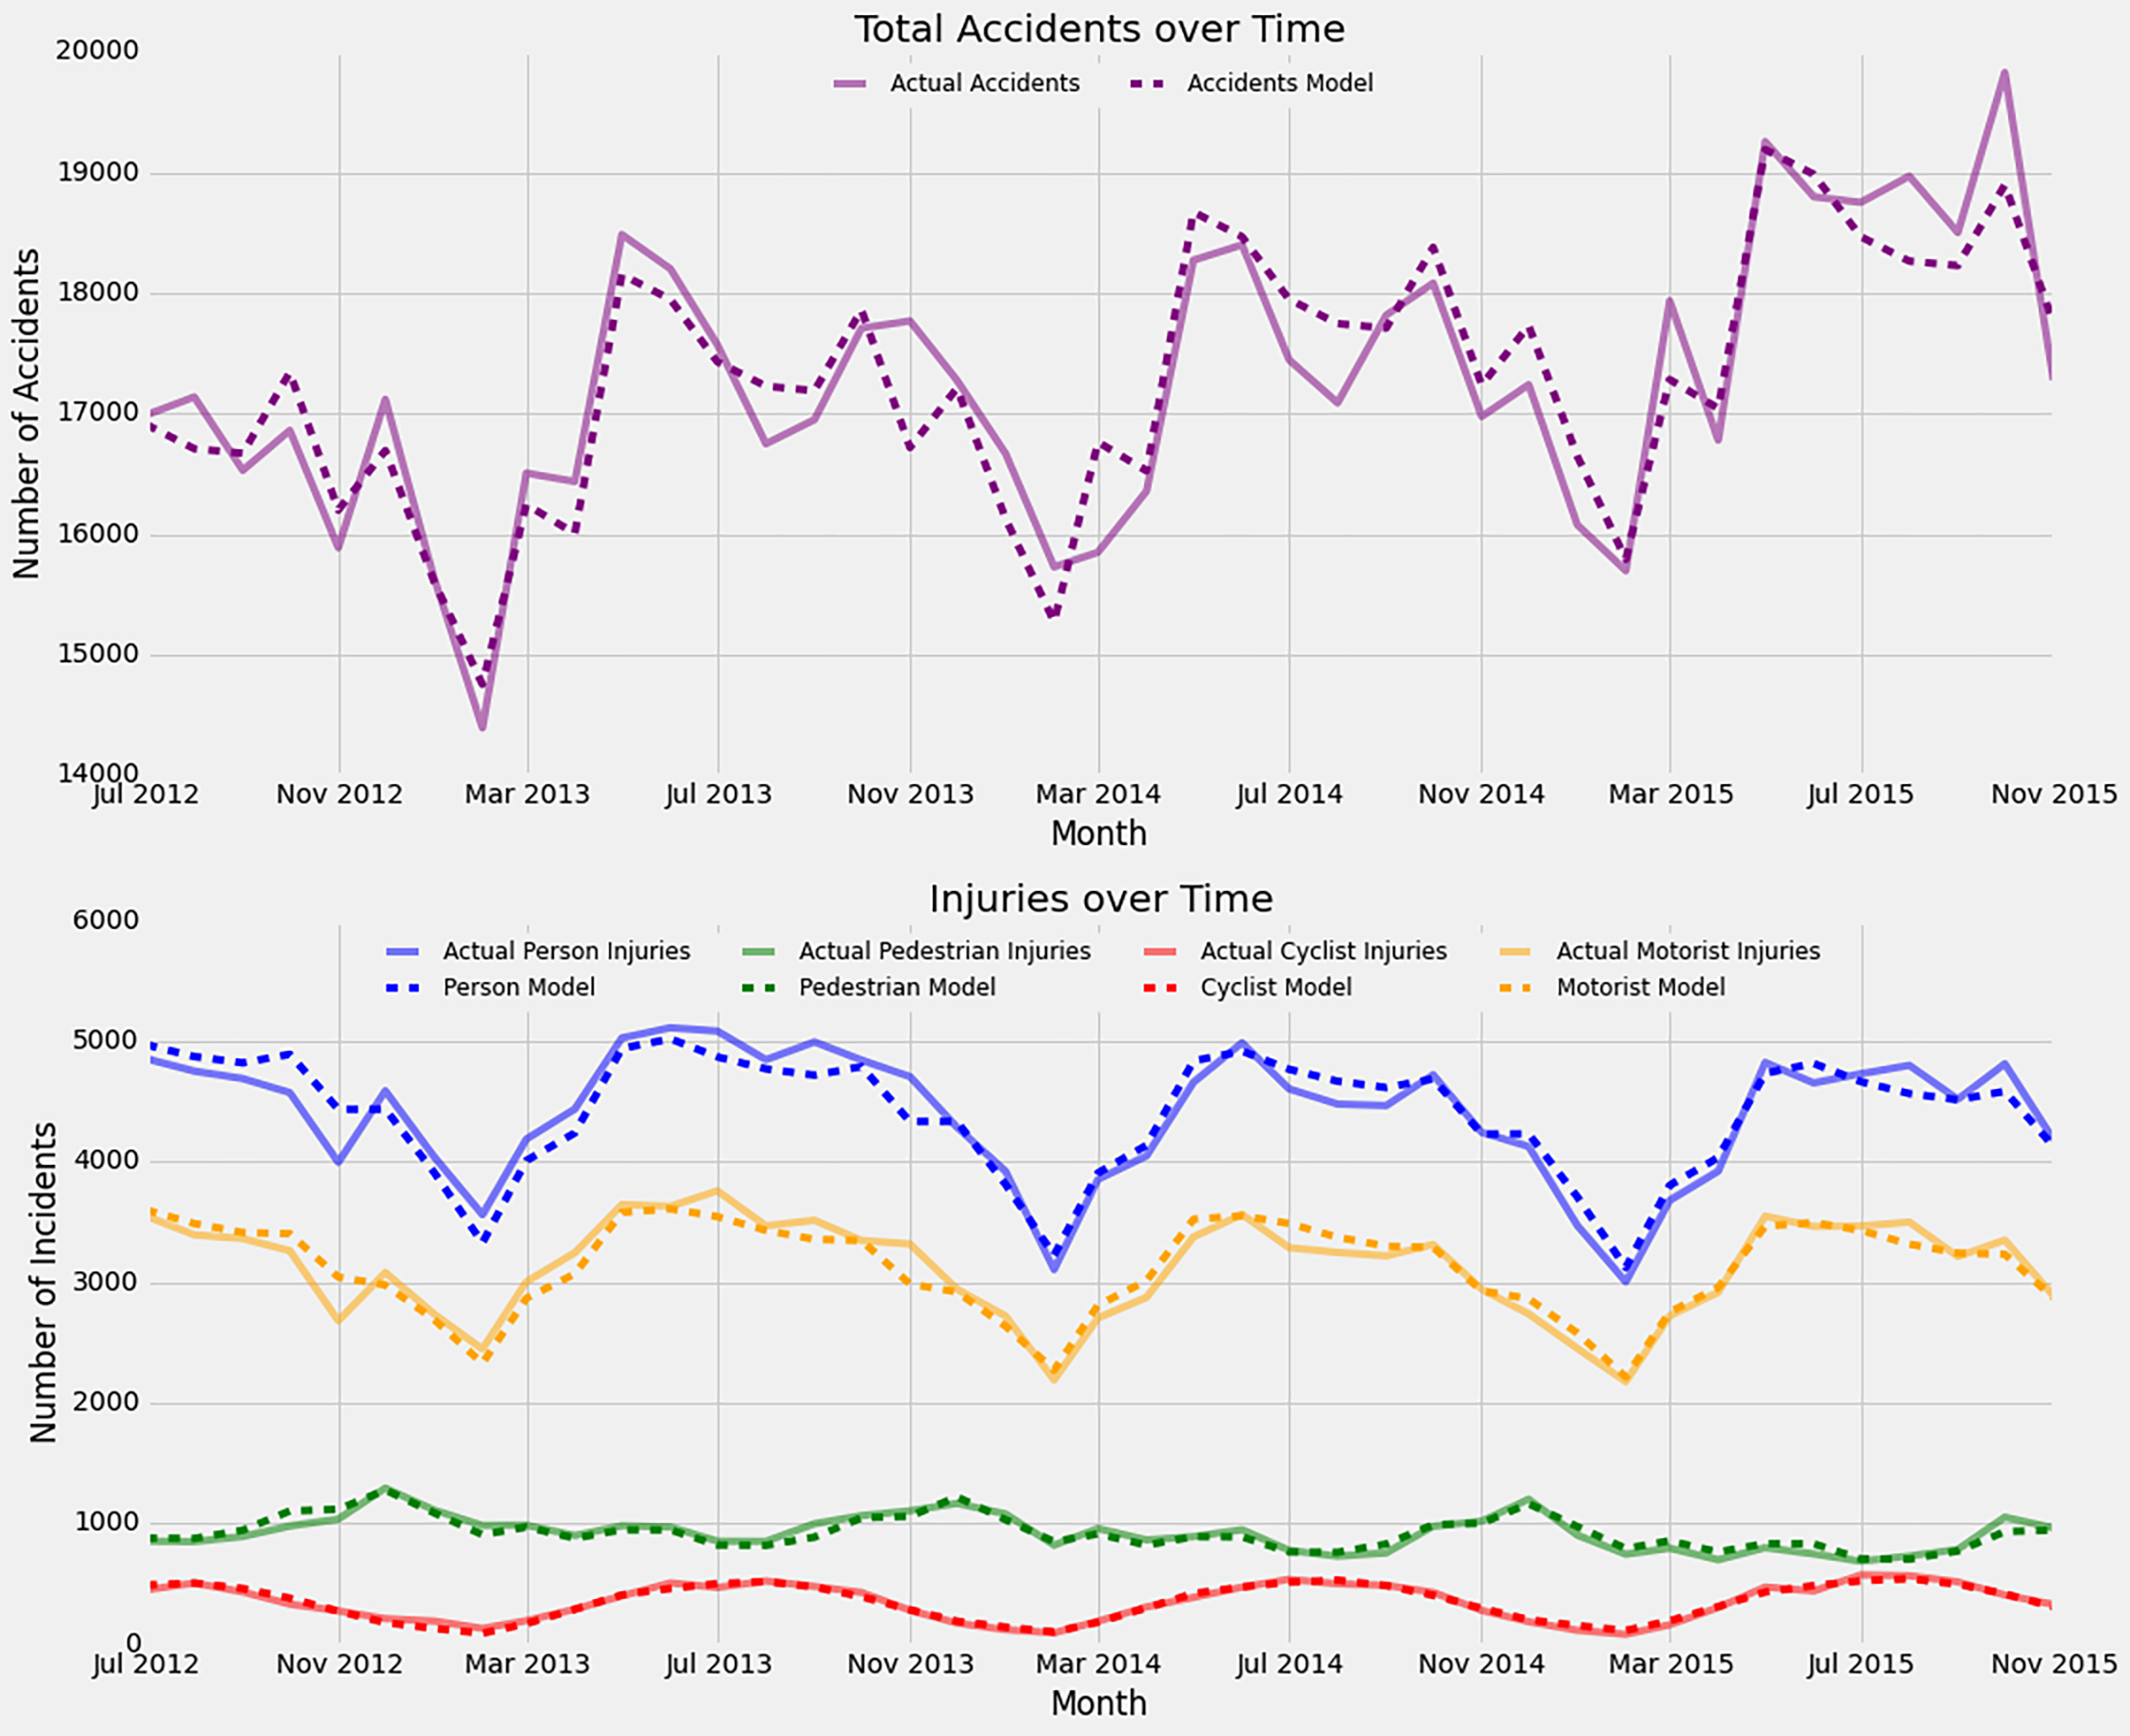
\includegraphics[width=\textwidth]{fig1.png}
	\caption{Timelines of total number of accidents and number of injuries over time for the whole dataset, aggregated by month.  An OLS regression was run on each using the month as a categorical variable and the elapsed months since July 2012.  In call cases a statistically signficant overall trend was found with total accidents increasing and all injury counts besides cyclists decreasing as detailed in Table \ref{tab:timeline}.}\label{fig:timeline}
\end{figure*}

\begin{table*}[]
\centering
\caption{Results from OLS linear regression of the number of accidents and injuries per month for the entire timeframe of the dataset.  Regression was done on the month as a categorical variable and the number of months since July 2012.  The time coefficent gives a measure of how many much the monthly total is increasing or decreasing per month.  All results were found to be significant to a .05 significance level.  Total number of accidents and cyclists injured trended upwards since July 2012 while total number of injuries, pedestrians injured and motorists injured trended donwards. }
\label{tab:timeline}
\begin{tabular}{|l|l|l|l|l|l|}
\hline
                    & R\textsuperscript{2}   & Time Coefficent & \multicolumn{2}{l|}{95\% Confidence Interval} & P-Value \\ \hline
Accidents           & .845 & 43.191          & 28.638                 & 57.744               & 0.000   \\ \hline
Persons Injured     & .890 & -8.519          & -14.202                & -2.836               & 0.005   \\ \hline
Pedestrians Injured & .864 & -4.769          & -6.512                 & -3.027               & 0.000   \\ \hline
Cyclists Injured    & .963 & 0.984           & 0.051                  & 1.917                & 0.039   \\ \hline
Motorists Injured   & .900 & -4.734          & -8.900                 & -0.568               & 0.027   \\ \hline
\end{tabular}
\end{table*}





%%%%%%%%%%%%%%%%%%%%%%LIT REVIEW %%%%%%%%%%%%%%%%%%%%%%%%%%%%%%

\section{Background}

It is a given that a collision occuring at higher speeds will be more serious than one at lower speeds because the kinetic energy law says that a vehicle's kinetic energy goes up in relation to the velocity squared. A pedestrian hit at 40mph has more than an 80\% chance to be killed, while only about 40\% chance when the car is going 30mph and just a 5\% chance to be killed at 20mph\cite{fatalityrates}.

The relationship between speed and likelihood of a collision is less clear. Studying a speed limit change in Sweden from 90kph to 110kph, Nilsson found that not only severity, but also number of crashes followed the kinetic energy model, so that the number of crashes change exponetially with the average traffic speed, which changes with the speed limit\cite{aarts2006driving}.  

A number of before and after studies for places such as Illinois\cite{rock1995impact} and Hong Kong\cite{wong2005would} also found similar increases to accidents, injuries and fatalities when speed limits were increased.

On the other hand, Solomon, Cirillo and others have found that the biggest indicator of accidents is not the maximum speed or average road speed, but the amount of speed dispersion between vehicles, with vehicles traveling signficantly above or below the average speed causing more accidents\cite{aarts2006driving}.  This is due to speed dispersion leading to more interactions between vehicles, each of which could lead to a collision.  

David Navon built a simulation to model the frequency of what he calls Accident Prone Interactions (APIs)  in relation to average traffic speed and found that at lower average speeds the number of the APIs was in increased compared to at higher speeds\cite{navon2003paradox}.  

There is also the question of whether speed limit changes actually impact driver behavior.  Wilmot and Khanal summarized findings that the speed drivers go at is changed very little based on a change in the speed limit.  The speed they choose to drive is more influenced by what they personally feel is a safe speed and less on the law.  The average speed of a roadway changes about 25\% of the speed limit changed.  This would imply just a 1-2mph change for New York City following the speed limit decrease.  Furthermore, the results are mixed, but some studies have found that decreaseing the speed limit increases the speed dispersion, likely due to some drivers following the new limit while others continuing to drive as before\cite{wilmot1999effect}.

The only thing that appears to be certain is that a lower \textit{actual} speed reduces the severity of collisions.  Beyond that there doesn't appear to be convincing evidence one way or the other that decreased speed limits decreases total number of accidents, injuries and fatalities.  It does from the models and findings of speed dispersion as a predictor of accidents, that because pedestrians can be thought of  as having essentially zero speed, that any decrease in the average speed of cars would lead to fewer pedestrian-vehicle collisions.  But pedestrian-vehicle collisions are only a portion of the total, so any change to decrease pedestrian collisions needs to be balanced with the impact to vehicle-vehicle collisions.

%%%%%%%%%%%%%%%%%DATA%%%%%%%%%%%%%%%%%%%%%%%%%%%%%

\section{Data}

\subsection{Vehicle Collisions}

The primary data used is the NYPD MotorVehicle Collisions dataset available on NYC Open Data\cite{crashdata}.  The dataset contains about 700,000 incident records from July 2012 through November 2015.  Of the 700,000 records, 600,000 are geolocated with latitude and longitude.  Each record has the number of injuries and fatalities for pedestrians, cyclists, motorists and in total.  It also contains information about the types of vehicles involved in the accidents, and contributing factors such as if the driver was drowsy or failed to yield right-of-way.

Overall the number of injuries is trending downward yet the number of accidents is actually trending upwards. Both also exhibit a strong seasonal trend. This was assessed by running an Ordinary least squares (OLS) regression on the monthly accident and injury counts versus the number of months since July 2012 and the month as a categorical variable. Figure \ref{fig:timeline} shows the timeline of accidents and injures for the dataset and Table \ref{tab:timeline} has regression results. The fatality counts prooved too noisy to see any statistically significant patterns over this time frame.



\subsection{Neighborhood Slow Zones}

The New York City Department of Transportation provides the geographic boundries of all current neighborhood slow zones in both geoJSON and shapefile formats\cite{slowzones}.  In this case the geoJSON format was used.  In addition to the geographic boundries, each record also contains the name of the slow zone and a year.  But this year is\textit{not} the year that the slow zone was put into place, instead it is the year that the plan was presented to the local community boards, which is not useful for our purpose.  Instead the year and month that each slowzone was put into place was compiled manually by the author based on new archives.  As such, it is likely error prone.  Appendix \ref{sec:appendixa} lists the dates used for this analysis.

\begin{figure*}[p]
	\centering
	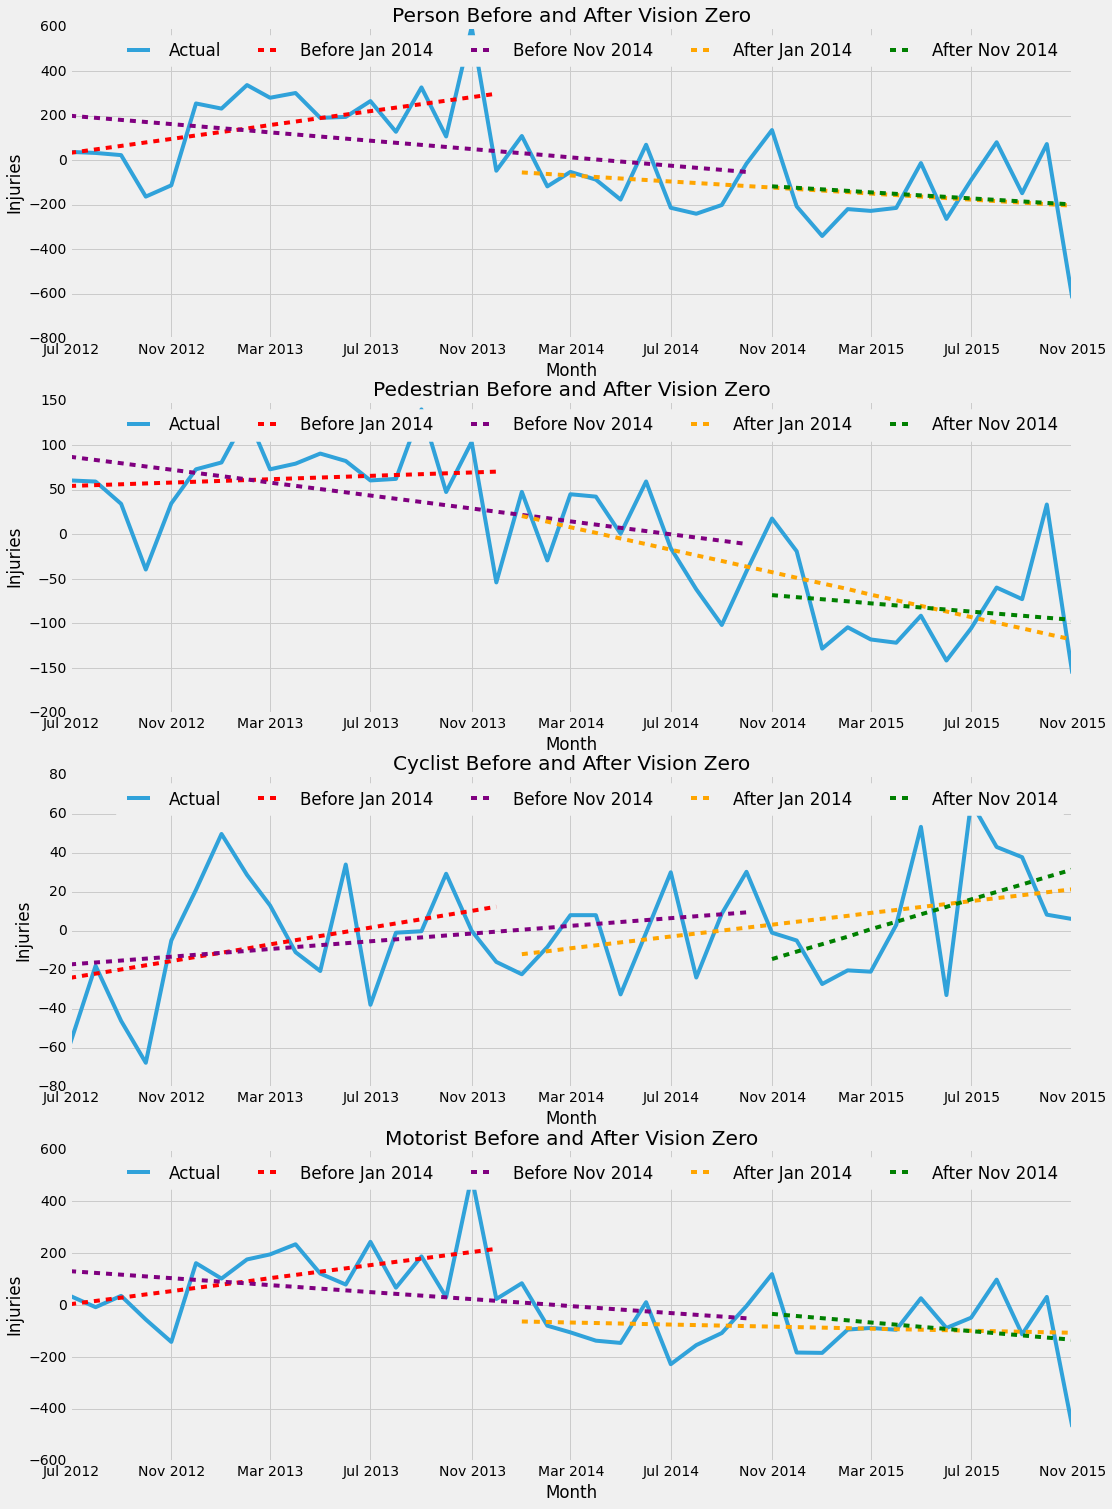
\includegraphics[width=\textwidth]{fig2.png}
	\caption{Before and after analysis for total injuries and by type of injury.  Analyzed before and after both January 2014, when Vision Zero started, and November 2014, when the speed limit was reduced to 25mph.  Actual is the number of injuries controlled for month.  No significant change was found for any category for either the January or November partition to a .05 significance level.  Regression results are detailed in Table \ref{tab:ana}.}\label{fig:injuryana}
\end{figure*}

\section{Analysis}
\subsection{City Wide Before and After Analysis}

\subsubsection{Methodology}

The total number of accidents and injuries by category (persons, pedestrians, cyclists and motorists) was analyzed before and after January 2014, when Vision Zero was first started, and before and after November 2014, when the citywide speed limit was decreased from 30mph to 25mph.  Therefore the four intervals we're interested in are July 2012 - January 2014, January 2014 - November 2015, July 2012 - November 2014 and November 2014 - November 2015.

For total accidents, and each category the data was aggregated by month, controlled for the month to remove the seasonal effect described above, and then a linear regression was run on each subinterval decribed above.  The confidence intervals for the coefficents were compared before and after for overlap.  If the coefficient of regression before has a non-overlapping confidence interval from the confidence interval of the coefficient after, then there is a significant chance that there has been  change in the rate of change of number of accidents or injuries from before to after.  On the other hand, if the two confidence intervals overlap, then we can't conclude that there has been such a change.

\subsubsection{Results}

Figures \ref{fig:totalana} and \ref{fig:injuryana} and Table \ref{tab:ana} summarize the results.  Split into the smaller time intervals, very few of the intervals had a statistically significant trend on their own, and none of the before intervals were disjoint from the after intervals.  Therefore we cannot conclude that either after the start of New York City Vision Zero, or after the speed limit decrease that there has been a stastically significant change in rate at which the total number of collisions or the number of injuries across the city as a whole is changing.  



\begin{figure*}[h]
	\centering
	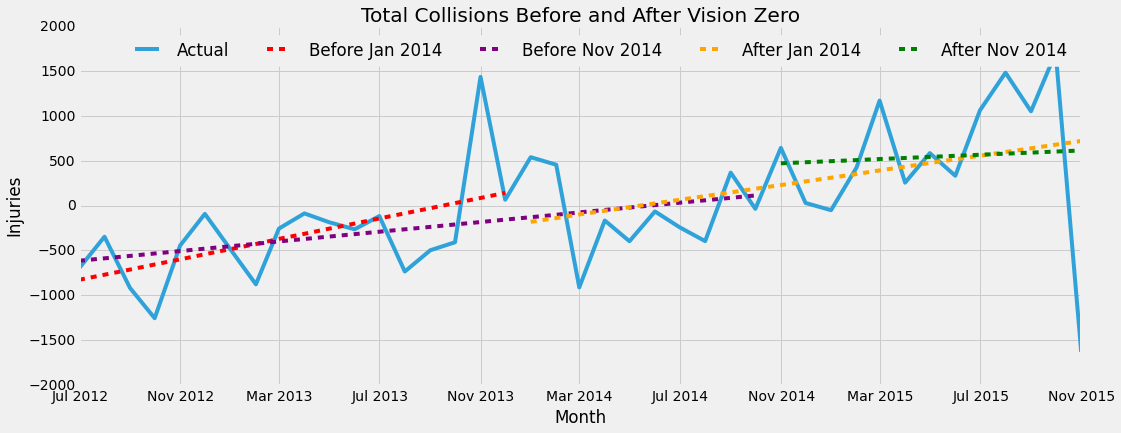
\includegraphics[width=\textwidth]{fig3.png}
	\caption{Before and after analysis for total number of collisions.  Analyzed before and after both January 2014, when Vision Zero started, and November 2014, when the speed limit was reduced to 25mph.  Actual is the number of collisions controlled for month.  No significant change was found for any category for either the January or November partition to a .05 significance level.  Regression results are detailed in Table \ref{tab:ana}.}\label{fig:totalana}
\end{figure*}


\begin{table*}[]
\centering
\caption{Results from before and after regression analysis for total number of collisions and injuries by category. Linear Regression was run on each subset of the data and for each of the subintervals and the confidence intervals were compared from before to after for overlap.  In all cases, the 95\% confidence interval before overlaps with it after, meaning we can't conclude any change from before to after. }
\label{tab:ana}
\begin{tabular}{|l|l|l|l|l|l|l|}
\hline
                                     &            & Coefficient & R\textsuperscript{2}    & \multicolumn{2}{l|}{95\% Confidence Interval} & P-Value \\ \hline
\multirow{4}{*}{Total Collisions}    & Before January 2014 & 57.064      & 0.295 & 10.359                 & 103.769              & 0.020   \\ \cline{2-7} 
                                     & During and After January 2014  & 40.980      & 0.134 & -6.311                 & 88.270               & 0.086   \\ \cline{2-7} 
                                     & Before November 2014 & 26.982      & 0.176 & 3.425                  & 50.540                & 0.026  \\ \cline{2-7} 
                                     & During and After November 2014  & 11.933      & 0.003 & -132.563               & 156.429              & 0.859   \\ \hline
\multirow{4}{*}{Persons Injured}     & Before January 2014 & 15.628      & 0.201 & -0.868                 & 32.125               & 0.062   \\ \cline{2-7} 
                                     & During and After January 2014  & -6.782      & 0.072 & -17.848                & 4.284                & 0.216   \\ \cline{2-7} 
                                     & Before November 2014 & -9.346      & 0.139 & -18.720                & 0.028                & 0.051   \\ \cline{2-7} 
                                     & During and After November 2014  & -6.778      & 0.017 & -41.051                & 27.496               & 0.672   \\ \hline
\multirow{4}{*}{Pedestrians Injured} & Before January 2014 & 0.946       & 0.011 & -3.881                 & 5.772                & 0.683   \\ \cline{2-7} 
                                     & During and After January 2014  & -6.304      & 0.392 & -9.865                 & -2.743               & 0.001   \\ \cline{2-7} 
                                     & Before November 2014 & -3.626      & 0.249 & -6.165                 & -1.087               & 0.249   \\ \cline{2-7} 
                                     & During and After November 2014  & -2.310      & 0.023 & -12.403                & 7.783                & 0.624   \\ \hline
\multirow{4}{*}{Motorists Injured}   & Before January 2014 & 12.539      & 0.228 & 0.321                  & 24.757               & 0.045   \\ \cline{2-7} 
                                     & During and After January 2014  & -1.973      & 0.011 & -10.327                & 6.381                & 0.628   \\ \cline{2-7} 
                                     & Before November 2014 & -6.720      & 0.125 & -13.879                & 0.438                & 0.065   \\ \cline{2-7} 
                                     & During and After November 2014  & -8.293      & 0.046 & -33.255                & 16.669               & 0.480   \\ \hline
\multirow{4}{*}{Cyclists Injured}    & Before January 2014 & 2.147       & 0.124 & -0.873                 & 5.168                & 0.151   \\ \cline{2-7} 
                                     & During and After January 2014  & 1.514       & 0.136 & -0.217                 & 3.245                & 0.083   \\ \cline{2-7} 
                                     & Before November 2014 & 0.989       & 0.080 & -0.365                 & 2.343                & 0.145   \\ \cline{2-7} 
                                     & During and After November 2014  & 3.8274      & 0.215 & -1.021                 & 8.675                & 0.110   \\ \hline
\end{tabular}
\end{table*}

\subsection{Slow Zone Analysis}

\subsubsection{Methodology}


First, all collisions which weren't geolocated with latitude and longitude were dropped, leaving about 600,000 collisions.  Then each one was geospatially joined with the boundries of the slow zones to see if it happened in one of the boundries.  If it did, the particular slowzone was noted.  Then using the approximate dates in \ref{sec:appendixa}, each of the collisions which happened in a slowzone was marked as happening either before or after the slowzone was established.

Two slowzones, Claremont and Mt. Eden were both disregarded because they were established before the start of the collisions dataset in July 2012.  Therefore there was no way to account for the conditions before those slowzones were created.  For each other slowzone in which there was data for before and after the establishment of the slowzone, the G-Test was used to test whether there is a statistically significant difference between the distribution of incidents within the slowzone boundry before and after the slowzone was established with the distribution of the rest of the city before and after that same date.  This was done for total number of accidents as well as each injury category.  The results are in Tables \ref{tab:sz} and \ref{tab:sz2}.

\subsubsection{Results}

\begin{table*}[]
\centering
\caption{Poop }
\label{tab:sz}
\begin{tabular}{|l|l|l|l|l|l|l|l|}
\hline
Slow Zone                                      & Date Established            & Category            & SZ Before & SZ After & NYC Before & NYC After & P-Value  \\ \hline
\multirow{4}{*}{Inwood}                        & \multirow{4}{*}{2012-09-01} & Total Collisions    & 28        & 480      & 29005      & 566648    & 0.575707 \\ \cline{3-8} 
                                               &                             & Motorist Injuries   & 1         & 46       & 5842       & 100047    & 0.450159 \\ \cline{3-8} 
                                               &                             & Pedestrian Injuries & 1         & 31       & 1544       & 32487     & 0.967243 \\ \cline{3-8} 
                                               &                             & Person Injuries     & 2         & 89       & 8262       & 144663    & 0.217994 \\ \hline
\multirow{3}{*}{Eastchester}                   & \multirow{3}{*}{2012-10-01} & Total Collisions    & 7         & 114      & 43101      & 552529    & 0.652047 \\ \cline{3-8} 
                                               &                             & Motorist Injuries   & 2         & 20       & 8603       & 97295     & 0.818009 \\ \cline{3-8} 
                                               &                             & Person Injuries     & 2         & 28       & 12241      & 140679    & 0.947413 \\ \hline
Riverdale                                      & 2012-10-01                  & Total Collisions    & 11        & 101      & 43101      & 552529    & 0.401945 \\ \hline
\multirow{5}{*}{Boerum Hill}                   & \multirow{5}{*}{2012-11-01} & Total Collisions    & 68        & 562      & 57389      & 538321    & 0.365990 \\ \cline{3-8} 
                                               &                             & Cyclist Injuries    & 2         & 25       & 1570       & 11437     & 0.642564 \\ \cline{3-8} 
                                               &                             & Motorist Injuries   & 10        & 61       & 11366      & 94539     & 0.485880 \\ \cline{3-8} 
                                               &                             & Pedestrian Injuries & 1         & 29       & 3253       & 30775     & 0.354236 \\ \cline{3-8} 
                                               &                             & Person Injuries     & 13        & 115      & 16189      & 136751    & 0.988850 \\ \hline
\multirow{4}{*}{Baychester}                    & \multirow{4}{*}{2012-12-01} & Total Collisions    & 36        & 294      & 70858      & 524803    & 0.635991 \\ \cline{3-8} 
                                               &                             & Motorist Injuries   & 14        & 88       & 13630      & 92273     & 0.912841 \\ \cline{3-8} 
                                               &                             & Pedestrian Injuries & 1         & 13       & 4185       & 29834     & 0.853851 \\ \cline{3-8} 
                                               &                             & Person Injuries     & 15        & 101      & 19640      & 133299    & 0.912017 \\ \hline
\multirow{4}{*}{Rosebank}                      & \multirow{4}{*}{2013-02-01} & Total Collisions    & 15        & 87       & 98713      & 496872    & 0.705023 \\ \cline{3-8} 
                                               &                             & Motorist Injuries   & 3         & 19       & 18456      & 87435     & 0.849214 \\ \cline{3-8} 
                                               &                             & Pedestrian Injuries & 2         & 5        & 6368       & 27647     & 0.856901 \\ \cline{3-8} 
                                               &                             & Person Injuries     & 5         & 25       & 27026      & 125898    & 0.924771 \\ \hline
\multirow{5}{*}{Elmhurst}                      & \multirow{5}{*}{2013-03-01} & Total Collisions    & 202       & 858      & 110984     & 484596    & 0.754850 \\ \cline{3-8} 
                                               &                             & Cyclist Injuries    & 15        & 49       & 2325       & 10696     & 0.333004 \\ \cline{3-8} 
                                               &                             & Motorist Injuries   & 28        & 58       & 20500      & 85398     & \textcolor{red}{0.005563} \\ \cline{3-8} 
                                               &                             & Pedestrian Injuries & 22        & 105      & 7254       & 26760     & 0.310928 \\ \cline{3-8} 
                                               &                             & Person Injuries     & 65        & 212      & 30079      & 122854    & 0.138679 \\ \hline
\multirow{5}{*}{Jackson Heights/East Elmhurst} & \multirow{5}{*}{2013-04-01} & Total Collisions    & 64        & 293      & 125058     & 470620    & 0.166860 \\ \cline{3-8} 
                                               &                             & Cyclist Injuries    & 1         & 4        & 2506       & 10508     & 0.570629 \\ \cline{3-8} 
                                               &                             & Motorist Injuries   & 16        & 74       & 23016      & 82893     & 0.425286 \\ \cline{3-8} 
                                               &                             & Pedestrian Injuries & 4         & 13       & 8153       & 25879     & 0.810214 \\ \cline{3-8} 
                                               &                             & Person Injuries     & 21        & 91       & 33675      & 119280    & 0.464377 \\ \hline
\multirow{4}{*}{Auburndale}                    & \multirow{4}{*}{2013-06-01} & Total Collisions    & 42        & 85       & 154876     & 440668    & 0.094523 \\ \cline{3-8} 
                                               &                             & Motorist Injuries   & 4         & 7        & 28924      & 76923     & 0.742132 \\ \cline{3-8} 
                                               &                             & Pedestrian Injuries & 1         & 1        & 9864       & 24162     & 0.899549 \\ \cline{3-8} 
                                               &                             & Person Injuries     & 5         & 9        & 41928      & 110958    & 0.697084 \\ \hline
\multirow{5}{*}{Corona}                        & \multirow{5}{*}{2013-06-01} & Total Collisions    & 179       & 556      & 154876     & 440668    & 0.324627 \\ \cline{3-8} 
                                               &                             & Cyclist Injuries    & 15        & 43       & 3140       & 9873      & 0.878201 \\ \cline{3-8} 
                                               &                             & Motorist Injuries   & 15        & 76       & 28924      & 76923     & \textcolor{red}{0.020797} \\ \cline{3-8} 
                                               &                             & Pedestrian Injuries & 21        & 58       & 9864       & 24162     & 0.727018 \\ \cline{3-8} 
                                               &                             & Person Injuries     & 51        & 177      & 41928      & 110958    & 0.095138 \\ \hline
\multirow{5}{*}{New Brighton / St George}      & \multirow{5}{*}{2013-06-01} & Total Collisions    & 81        & 258      & 154876     & 440668    & 0.405801 \\ \cline{3-8} 
                                               &                             & Cyclist Injuries    & 1         & 5        & 3140       & 9873      & 0.960257 \\ \cline{3-8} 
                                               &                             & Motorist Injuries   & 8         & 31       & 28924      & 76923     & 0.427581 \\ \cline{3-8} 
                                               &                             & Pedestrian Injuries & 9         & 16       & 9864       & 24162     & 0.586950 \\ \cline{3-8} 
                                               &                             & Person Injuries     & 18        & 52       & 41928      & 110958    & 0.851379 \\ \hline
\multirow{4}{*}{Dongan Hills}                  & \multirow{4}{*}{2013-09-01} & Total Collisions    & 128       & 193      & 198949     & 396732    & \textcolor{red}{0.017909} \\ \cline{3-8} 
                                               &                             & Motorist Injuries   & 18        & 37       & 37898      & 67951     & 0.736344 \\ \cline{3-8} 
                                               &                             & Pedestrian Injuries & 4         & 9        & 12285      & 21739     & 0.910683 \\ \cline{3-8} 
                                               &                             & Person Injuries     & 22        & 50       & 54683      & 98204     & 0.419288 \\ \hline
\multirow{5}{*}{Norwood}                       & \multirow{5}{*}{2014-06-01} & Total Collisions    & 367       & 349      & 326781     & 268806    & 0.057583 \\ \cline{3-8} 
                                               &                             & Cyclist Injuries    & 1         & 7        & 6762       & 6248      & 0.052058 \\ \cline{3-8} 
                                               &                             & Motorist Injuries   & 69        & 46       & 59918      & 45944     & 0.520210 \\ \cline{3-8} 
                                               &                             & Pedestrian Injuries & 29        & 17       & 20296      & 13719     & 0.751206 \\ \cline{3-8} 
                                               &                             & Person Injuries     & 99        & 70       & 86976      & 65911     & 0.714070 \\ \hline
\end{tabular}
\end{table*}

\begin{table*}[]
\centering
\caption{Table \ref{tab:sz} Continued}
\label{tab:sz2}
\begin{tabular}{|l|l|l|l|l|l|l|l|}
\hline
Slow Zone                                   & Date Established            & Category            & SZ Before & SZ After & NYC Before & NYC After & P-Value  \\ \hline
\multirow{5}{*}{Alphabet City Tompkins}     & \multirow{5}{*}{2014-08-01} & Total Collisions    & 1117      & 710      & 356801     & 238711    & 0.296788 \\ \cline{3-8} 
                                            &                             & Cyclist Injuries    & 93        & 46       & 7691       & 5317      & 0.073407 \\ \cline{3-8} 
                                            &                             & Motorist Injuries   & 81        & 59       & 65534      & 40332     & 0.371908 \\ \cline{3-8} 
                                            &                             & Pedestrian Injuries & 121       & 67       & 21859      & 12154     & 0.960796 \\ \cline{3-8} 
                                            &                             & Person Injuries     & 295       & 172      & 95084      & 57803     & 0.698405 \\ \hline
\multirow{5}{*}{Jackson Heights}            & \multirow{5}{*}{2014-09-01} & Total Collisions    & 1064      & 635      & 371079     & 224671    & 0.793639 \\ \cline{3-8} 
                                            &                             & Cyclist Injuries    & 47        & 25       & 8157       & 4854      & 0.740453 \\ \cline{3-8} 
                                            &                             & Motorist Injuries   & 112       & 72       & 68195      & 37712     & 0.360751 \\ \cline{3-8} 
                                            &                             & Pedestrian Injuries & 81        & 45       & 22520      & 11514     & 0.725991 \\ \cline{3-8} 
                                            &                             & Person Injuries     & 240       & 142      & 98872      & 54080     & 0.493199 \\ \hline
\multirow{5}{*}{Sunnyside Gardens-Woodside} & \multirow{5}{*}{2015-08-01} & Total Collisions    & 611       & 58       & 533209     & 62301     & 0.136666 \\ \cline{3-8} 
                                            &                             & Cyclist Injuries    & 28        & 3        & 11362      & 1651      & 0.812932 \\ \cline{3-8} 
                                            &                             & Motorist Injuries   & 72        & 4        & 95363      & 10500     & 0.210980 \\ \cline{3-8} 
                                            &                             & Pedestrian Injuries & 67        & 4        & 30883      & 3142      & 0.374625 \\ \cline{3-8} 
                                            &                             & Person Injuries     & 167       & 11       & 137608     & 15293     & 0.094482 \\ \hline
\multirow{5}{*}{Sunnyside}                  & \multirow{5}{*}{2015-08-01} & Total Collisions    & 912       & 70       & 533209     & 62301     & \textcolor{red}{0.000401} \\ \cline{3-8} 
                                            &                             & Cyclist Injuries    & 17        & 5        & 11362      & 1651      & 0.309135 \\ \cline{3-8} 
                                            &                             & Motorist Injuries   & 150       & 8        & 95363      & 10500     & \textcolor{red}{0.038299} \\ \cline{3-8} 
                                            &                             & Pedestrian Injuries & 59        & 1        & 30883      & 3142      & \textcolor{red}{0.034966} \\ \cline{3-8} 
                                            &                             & Person Injuries     & 226       & 14       & 137608     & 15293     & \textcolor{red}{0.028537} \\ \hline
\multirow{5}{*}{Astoria}                    & \multirow{5}{*}{2015-09-01} & Total Collisions    & 851       & 68       & 549153     & 46395     & 0.701842 \\ \cline{3-8} 
                                            &                             & Cyclist Injuries    & 38        & 4        & 11871      & 1137      & 0.924404 \\ \cline{3-8} 
                                            &                             & Motorist Injuries   & 94        & 7        & 98183      & 7711      & 0.955614 \\ \cline{3-8} 
                                            &                             & Pedestrian Injuries & 64        & 5        & 31543      & 2474      & 0.825554 \\ \cline{3-8} 
                                            &                             & Person Injuries     & 196       & 16       & 141597     & 11322     & 0.958738 \\ \hline
\multirow{4}{*}{Brooklyn Heights}           & \multirow{4}{*}{2015-10-01} & Total Collisions    & 1328      & 55       & 564801     & 30706     & \textcolor{red}{0.046077} \\ \cline{3-8} 
                                            &                             & Motorist Injuries   & 127       & 2        & 100851     & 5038      & 0.089264 \\ \cline{3-8} 
                                            &                             & Pedestrian Injuries & 49        & 1        & 32243      & 1764      & 0.451011 \\ \cline{3-8} 
                                            &                             & Person Injuries     & 191       & 3        & 145436     & 7468      & \textcolor{red}{0.023053} \\ \hline
\multirow{5}{*}{Prospect Heights}           & \multirow{5}{*}{2015-10-01} & Total Collisions    & 793       & 41       & 564801     & 30706     & 0.813087 \\ \cline{3-8} 
                                            &                             & Cyclist Injuries    & 49        & 3        & 12342      & 666       & 0.917007 \\ \cline{3-8} 
                                            &                             & Motorist Injuries   & 112       & 4        & 100851     & 5038      & 0.646852 \\ \cline{3-8} 
                                            &                             & Pedestrian Injuries & 59        & 1        & 32243      & 1764      & 0.299220 \\ \cline{3-8} 
                                            &                             & Person Injuries     & 220       & 8        & 145436     & 7468      & 0.399290 \\ \hline
\end{tabular}
\end{table*}

This analysis assumes that a small section of the city, when no special traffic infrastrucutre changes are made to that section, should exhibit the same patterns and trends as the rest of the city as a whole.  But traffic accidents are as much a factor of the infrastructure and policy as they are a factor of usage.  So as a neighborhood changes in population or makeup, we would expect traffic accidents to be affected.  But unfortunately there is no data (at least publically available) that provides numbers into how road and sidewalk usage has changed, so that factor couldn't be controlled for.  This assumption could be tested to some extent by taking random geographic samples and seeing if they on average follow the same trend as the city as a whole.  Also, as noted previously, the actual dates for when the slowzones were created are not available.

Given these limitations, there are still a couple of clear success stories that emerge - Sunnyside and Brooklyn Heights.  Both saw statistically significant drops in total collisions and total injuries after the establishment of the slowzones.  Sunside also saw a statistically significant drop in the number of pedestrian and motorist injuries.  Recall that a slowzone is actually composed of several different measures such as signage and speed humps and not just the decreased speed limit, so further research is necessary to determine what makes these two slowzones standout from the rest.

Oddly, though not statisically significant, the number of cyclist injuries in Sunnyside is up compared to the rest of the city after the slowzone was created.  Anecdotaly, speed humps can cause increased danger to cyclists, so there could be a connection there. 

\section{Conclusion}
These findings show that Vision Zero may be having an effect, but the results are not statistically significant.  But under the moral premise of Vision Zero, where lives should be saved at any cost, that might be enough to support the efforts.  HKDJUFLKDSFJ Rephrase this.

Lorem ipsum dolor sit amet, consectetur adipiscing elit, sed do eiusmod tempor incididunt ut labore et dolore magna aliqua. Ut enim ad minim veniam, quis nostrud exercitation ullamco laboris nisi ut aliquip ex ea commodo consequat. Duis aute irure dolor in reprehenderit in voluptate velit esse cillum dolore eu fugiat nulla pariatur. Excepteur sint occaecat cupidatat non proident, sunt in culpa qui officia deserunt mollit anim id est laborum.Lorem ipsum dolor sit amet, consectetur adipiscing elit, sed do eiusmod tempor incididunt ut labore et dolore magna aliqua. Ut enim ad minim veniam, quis nostrud exercitation ullamco laboris nisi ut aliquip ex ea commodo consequat. Duis aute irure dolor in reprehenderit in voluptate velit esse cillum dolore eu fugiat nulla pariatur. Excepteur sint occaecat cupidatat non proident, sunt in culpa qui officia deserunt mollit anim id est laborum.Lorem ipsum dolor sit amet, consectetur adipiscing elit, sed do eiusmod tempor incididunt ut labore et dolore magna aliqua. Ut enim ad minim veniam, quis nostrud exercitation ullamco laboris nisi ut aliquip ex ea commodo consequat. Duis aute irure dolor in reprehenderit in voluptate velit esse cillum dolore eu fugiat nulla pariatur. Excepteur sint occaecat cupidatat non proident, sunt in culpa qui officia deserunt mollit anim id est laborum.Lorem ipsum dolor sit amet, consectetur adipiscing elit, sed do eiusmod tempor incididunt ut labore et dolore magna aliqua. Ut enim ad minim veniam, quis nostrud exercitation ullamco laboris nisi ut aliquip ex ea commodo consequat. Duis aute irure dolor in reprehenderit in voluptate velit esse cillum dolore eu fugiat nulla pariatur. Excepteur sint occaecat cupidatat non proident, sunt in culpa qui officia deserunt mollit anim id est laborum.Lorem ipsum dolor sit amet, consectetur adipiscing elit, sed do eiusmod tempor incididunt ut labore et dolore magna aliqua. Ut enim ad minim veniam, quis nostrud exercitation ullamco laboris nisi ut aliquip ex ea commodo consequat. Duis aute irure dolor in reprehenderit in voluptate velit esse cillum dolore eu fugiat nulla pariatur. Excepteur sint occaecat cupidatat non proident, sunt in culpa qui officia deserunt mollit anim id est laborum.Lorem ipsum dolor sit amet, consectetur adipiscing elit, sed do eiusmod tempor incididunt ut labore et dolore magna aliqua. Ut enim ad minim veniam, quis nostrud exercitation ullamco laboris nisi ut aliquip ex ea commodo consequat. Duis aute irure dolor in reprehenderit in voluptate velit esse cillum dolore eu fugiat nulla pariatur. Excepteur sint occaecat cupidatat non proident, sunt in culpa qui officia deserunt mollit anim id est laborum.Lorem ipsum dolor sit amet, consectetur adipiscing elit, sed do eiusmod tempor incididunt ut labore et dolore magna aliqua. Ut enim ad minim veniam, quis nostrud exercitation ullamco laboris nisi ut aliquip ex ea commodo consequat. Duis aute irure dolor in reprehenderit in voluptate velit esse cillum dolore eu fugiat nulla pariatur. Excepteur sint occaecat cupidatat non proident, sunt in culpa qui officia deserunt mollit anim id est laborum.Lorem ipsum dolor sit amet, consectetur adipiscing elit, sed do eiusmod tempor incididunt ut labore et dolore magna aliqua. Ut enim ad minim veniam, quis nostrud exercitation ullamco laboris nisi ut aliquip ex ea commodo consequat. Duis aute irure dolor in reprehenderit in voluptate velit esse cillum dolore eu fugiat nulla pariatur. Excepteur sint occaecat cupidatat non proident, sunt in culpa qui officia deserunt mollit anim id est laborum.Lorem ipsum dolor sit amet, consectetur adipiscing elit, sed do eiusmod tempor incididunt ut labore et dolore magna aliqua. Ut enim ad minim veniam, quis nostrud exercitation ullamco laboris nisi ut aliquip ex ea commodo consequat. Duis aute irure dolor in reprehenderit in voluptate velit esse cillum dolore eu fugiat nulla pariatur. Excepteur sint occaecat cupidatat non proident, sunt in culpa qui officia deserunt mollit anim id est laborum.



% if have a single appendix:
%\appendix[Proof of the Zonklar Equations]
% or
%\appendix  % for no appendix heading
% do not use \section anymore after \appendix, only \section*
% is possibly needed

% use appendices with more than one appendix
% then use \section to start each appendix
% you must declare a \section before using any
% \subsection or using \label (\appendices by itself
% starts a section numbered zero.)
%


\appendices
\section{Slowzone Installation Dates}
\label{sec:appendixa}
\begin{table}[h!]
\centering

\caption*{Approximate year and month that the slowzone was installed.  Dates manually compiled by the author based on news archives. }

\begin{tabular}{|l|l|}
\hline
                                  Name &  Date \\ \hline
                          Claremont &  Nov 2011 \\ \hline
                            MT Eden &  Jul 2012 \\ \hline
                             Inwood &  Sep 2012 \\ \hline
                        Eastchester &  Oct 2012 \\ \hline
                          Riverdale &  Oct 2012 \\ \hline
                        Boerum Hill &  Nov 2012 \\ \hline
                         Baychester &  Dec 2012 \\ \hline
                           Rosebank &  Feb 2013 \\ \hline
                           Elmhurst &  Mar 2013 \\ \hline
      Jackson Heights/East Elmhurst &  Apr 2013 \\ \hline
           New Brighton / St George &  Jun 2013 \\ \hline
                         Auburndale &  Jun 2013 \\ \hline
                             Corona &  Jun 2013 \\ \hline
                       Dongan Hills &  Sep 2013 \\ \hline
                           Norwood &  Jun 2014 \\ \hline
 Alphabet City Tompkins Square Park &  Aug 2014 \\ \hline
                    Jackson Heights &  Sep 2014 \\ \hline
         Sunnyside Gardens-Woodside &  Aug 2015 \\ \hline
                          Sunnyside &  Aug 2015 \\ \hline
                            Astoria &  Sep 2015 \\ \hline
                   Prospect Heights &  Oct 2015 \\ \hline
                   Brooklyn Heights &  Oct 2015 \\ \hline
\end{tabular}
\end{table}



% use section* for acknowledgment
\ifCLASSOPTIONcompsoc
  % The Computer Society usually uses the plural form
  \section*{Acknowledgments}
\else
  % regular IEEE prefers the singular form
  \section*{Acknowledgment}
\fi


The authors would like to thank their cats Sweetie, Secondi, Kitten, Ubuntu, Collard Green, iOS, Mini Triangle Face, Euclid, Pythagoras, Isosceles and Tetra for all of the support they've provided.


% Can use something like this to put references on a page
% by themselves when using endfloat and the captionsoff option.
\ifCLASSOPTIONcaptionsoff
  \newpage
\fi



% trigger a \newpage just before the given reference
% number - used to balance the columns on the last page
% adjust value as needed - may need to be readjusted if
% the document is modified later
%\IEEEtriggeratref{8}
% The "triggered" command can be changed if desired:
%\IEEEtriggercmd{\enlargethispage{-5in}}

% references section

% can use a bibliography generated by BibTeX as a .bbl file
% BibTeX documentation can be easily obtained at:
% http://mirror.ctan.org/biblio/bibtex/contrib/doc/
% The IEEEtran BibTeX style support page is at:
% http://www.michaelshell.org/tex/ieeetran/bibtex/
%\bibliographystyle{apalike}
% argument is your BibTeX string definitions and bibliography database(s)
%\bibliography{IEEEabrv,../bib/paper}
%
% <OR> manually copy in the resultant .bbl file
% set second argument of \begin to the number of references
% (used to reserve space for the reference number labels box)


\bibliography{tingvall2000vision,vzreport,crashdata,fatalityrates,slowzones,aarts2006driving,wilmot1999effect,rock1995impact,wong2005would,navon2003paradox}


\end{document}


